\section{Main contributions}\label{contributions}

This section describes the main contributions of this thesis towards reducing the accidental complexity and the cost of UI development.

\subsection{Methods}\label{usecases}

The usage of a UI by a user consists of either \textbf{reading} or \textbf{interacting}. In terms of systems we can call them \textbf{querying} or \textbf{interacting} respectively.
I implement the proof-of-concept of the UI framework by incrementally implementing both capabilities.

\begin{enumerate}
  \item Query: The user is able to retrieve information from the UI by looking at it
  \item Interacting: The user is able to interact with the UI
\end{enumerate}

The development of the UI framework is driven by these two capabilities.

\subsection{Design goals}\label{basevocab}

Following design goals should be met by the UI framework.

\subsubsection{Play nicely with others}\label{usecases}

The most important design goal is to play nicely with others. We achieve that by conforming to web standards and making use of existing and established tooling. This design goal drove the choice of JSON-LD as serialization format for linked data.

JSON-LD allows us to stay compatible with all tools consuming and producing JSON.

\subsubsection{Upgrade path}\label{usecases}

By playing nicely with others, the UI framework is able to provide an upgrade path to already existing APIs.

\subsubsection{Customizability}\label{usecases}

\subsubsection{Developer ergonomics}\label{usecases}

\subsection{Use Case 1: Apartment}\label{usecases}

For the user to be able to query data, the UI has to render it.

The first use case describes a scenario in home automation. Several thermometers in several rooms in an apartment send the current temperature to a server. The goal is to develop a UI that displays apartments, rooms, and thermometers and temperatures in a sensible manner.

\begin{figure}[!htb]
  \center{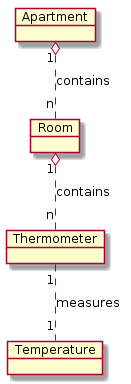
\includegraphics[width=100]
    {diagrams/iot.png}}
  \caption{\label{fig:my-label} Data model of the home automation use case.}
\end{figure}

\subsection{Use Case 2: Kanban Board}\label{usecases}

\subsection{Base vocabulary}\label{basevocab}

There are things and list of things. Base vocabulary is hydra.

\subsection{Generic rendering}\label{genericrendering}

There is linked data renderer, all the behavior is done by plugging in the custom renderer.

\subsection{Pluggable domain rendering}\label{domainrendering}

TODO show tree of data and application of renderer step by step

\subsection{User interaction}\label{interaction}

\subsubsection{Task based computing}\label{interaction}

TODO three types of operations:

inline operations
supported operations for all of the resource's types
supported operations for the supported property, where the resource is an object of said property

\subsubsection{CQRS}\label{interaction}
